% Copied from Gates-rebuild/figures/hypercube6_code.tex (generated by scripts/gen_hypercube6_tikz.py).
% Only the tikzpicture is kept, recolored to the deck palette: T gold, T-dagger teal.
% Vertex BbVv is block b (w=10,01,11) and u with u_i = bit i-1 of v.
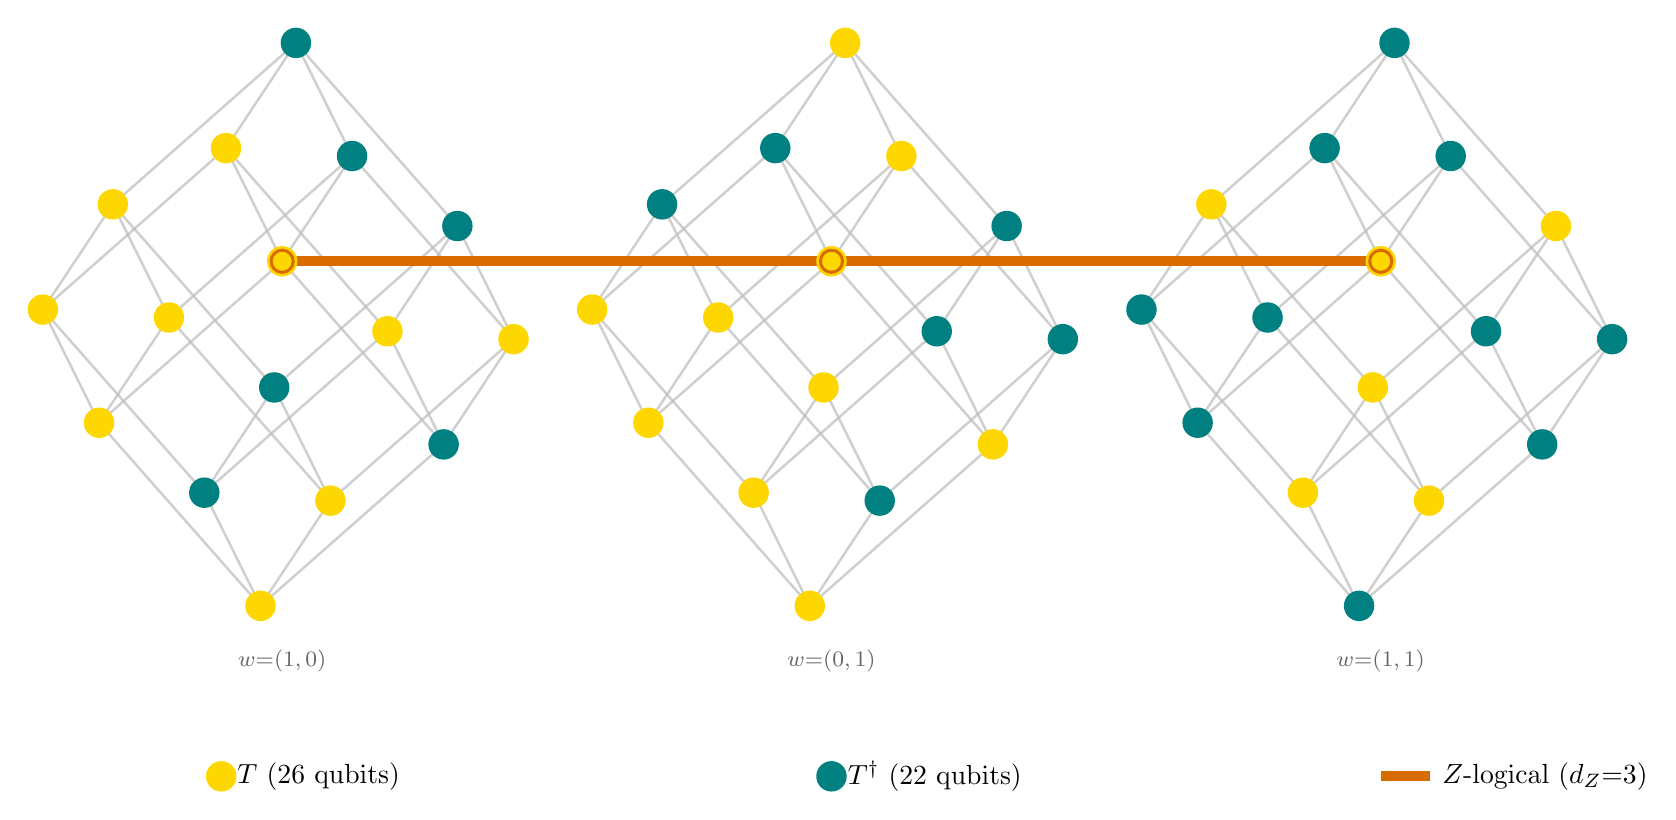
\begin{tikzpicture}[scale=1.55,
    every node/.style={inner sep=0pt},
    edge hyper/.style={line width=0.9pt, gray!50, opacity=0.75},
    vert T/.style={fill=Gold, circle, minimum size=11pt},
    vert Tdag/.style={fill=Teal, circle, minimum size=11pt},
    vert Zhigh/.style={circle, minimum size=8pt, line width=1.1pt},
    zlogical/.style={line width=3.5pt, orange!85!black},
    block label/.style={font=\footnotesize\sffamily, text=black!60},
    legend label/.style={font=\normalsize},
]

% --- Vertex coordinates (3 blocks of 16) ---
\coordinate (B0V0) at (-4.5000, 0.0000);
\coordinate (B0V1) at (-3.9272, 0.8621);
\coordinate (B0V2) at (-3.1774, -1.5002);
\coordinate (B0V3) at (-2.6046, -0.6381);
\coordinate (B0V4) at (-6.0002, -1.3226);
\coordinate (B0V5) at (-5.4275, -0.4606);
\coordinate (B0V6) at (-4.6776, -2.8228);
\coordinate (B0V7) at (-4.1048, -1.9608);
\coordinate (B0V8) at (-4.9602, 0.9271);
\coordinate (B0V9) at (-4.3874, 1.7891);
\coordinate (B0V10) at (-3.6376, -0.5732);
\coordinate (B0V11) at (-3.0648, 0.2889);
\coordinate (B0V12) at (-6.4604, -0.3956);
\coordinate (B0V13) at (-5.8877, 0.4665);
\coordinate (B0V14) at (-5.1378, -1.8958);
\coordinate (B0V15) at (-4.5650, -1.0337);
\coordinate (B1V0) at (0.0000, 0.0000);
\coordinate (B1V1) at (0.5728, 0.8621);
\coordinate (B1V2) at (1.3226, -1.5002);
\coordinate (B1V3) at (1.8954, -0.6381);
\coordinate (B1V4) at (-1.5002, -1.3226);
\coordinate (B1V5) at (-0.9275, -0.4606);
\coordinate (B1V6) at (-0.1776, -2.8228);
\coordinate (B1V7) at (0.3952, -1.9608);
\coordinate (B1V8) at (-0.4602, 0.9271);
\coordinate (B1V9) at (0.1126, 1.7891);
\coordinate (B1V10) at (0.8624, -0.5732);
\coordinate (B1V11) at (1.4352, 0.2889);
\coordinate (B1V12) at (-1.9604, -0.3956);
\coordinate (B1V13) at (-1.3877, 0.4665);
\coordinate (B1V14) at (-0.6378, -1.8958);
\coordinate (B1V15) at (-0.0650, -1.0337);
\coordinate (B2V0) at (4.5000, 0.0000);
\coordinate (B2V1) at (5.0728, 0.8621);
\coordinate (B2V2) at (5.8226, -1.5002);
\coordinate (B2V3) at (6.3954, -0.6381);
\coordinate (B2V4) at (2.9998, -1.3226);
\coordinate (B2V5) at (3.5725, -0.4606);
\coordinate (B2V6) at (4.3224, -2.8228);
\coordinate (B2V7) at (4.8952, -1.9608);
\coordinate (B2V8) at (4.0398, 0.9271);
\coordinate (B2V9) at (4.6126, 1.7891);
\coordinate (B2V10) at (5.3624, -0.5732);
\coordinate (B2V11) at (5.9352, 0.2889);
\coordinate (B2V12) at (2.5396, -0.3956);
\coordinate (B2V13) at (3.1123, 0.4665);
\coordinate (B2V14) at (3.8622, -1.8958);
\coordinate (B2V15) at (4.4350, -1.0337);

% --- Hypercube edges (4-cube skeleton per block) ---
\draw[edge hyper] (B0V0) -- (B0V1);
\draw[edge hyper] (B0V0) -- (B0V2);
\draw[edge hyper] (B0V0) -- (B0V4);
\draw[edge hyper] (B0V0) -- (B0V8);
\draw[edge hyper] (B0V1) -- (B0V3);
\draw[edge hyper] (B0V1) -- (B0V5);
\draw[edge hyper] (B0V1) -- (B0V9);
\draw[edge hyper] (B0V2) -- (B0V3);
\draw[edge hyper] (B0V2) -- (B0V6);
\draw[edge hyper] (B0V2) -- (B0V10);
\draw[edge hyper] (B0V3) -- (B0V7);
\draw[edge hyper] (B0V3) -- (B0V11);
\draw[edge hyper] (B0V4) -- (B0V5);
\draw[edge hyper] (B0V4) -- (B0V6);
\draw[edge hyper] (B0V4) -- (B0V12);
\draw[edge hyper] (B0V5) -- (B0V7);
\draw[edge hyper] (B0V5) -- (B0V13);
\draw[edge hyper] (B0V6) -- (B0V7);
\draw[edge hyper] (B0V6) -- (B0V14);
\draw[edge hyper] (B0V7) -- (B0V15);
\draw[edge hyper] (B0V8) -- (B0V9);
\draw[edge hyper] (B0V8) -- (B0V10);
\draw[edge hyper] (B0V8) -- (B0V12);
\draw[edge hyper] (B0V9) -- (B0V11);
\draw[edge hyper] (B0V9) -- (B0V13);
\draw[edge hyper] (B0V10) -- (B0V11);
\draw[edge hyper] (B0V10) -- (B0V14);
\draw[edge hyper] (B0V11) -- (B0V15);
\draw[edge hyper] (B0V12) -- (B0V13);
\draw[edge hyper] (B0V12) -- (B0V14);
\draw[edge hyper] (B0V13) -- (B0V15);
\draw[edge hyper] (B0V14) -- (B0V15);
\draw[edge hyper] (B1V0) -- (B1V1);
\draw[edge hyper] (B1V0) -- (B1V2);
\draw[edge hyper] (B1V0) -- (B1V4);
\draw[edge hyper] (B1V0) -- (B1V8);
\draw[edge hyper] (B1V1) -- (B1V3);
\draw[edge hyper] (B1V1) -- (B1V5);
\draw[edge hyper] (B1V1) -- (B1V9);
\draw[edge hyper] (B1V2) -- (B1V3);
\draw[edge hyper] (B1V2) -- (B1V6);
\draw[edge hyper] (B1V2) -- (B1V10);
\draw[edge hyper] (B1V3) -- (B1V7);
\draw[edge hyper] (B1V3) -- (B1V11);
\draw[edge hyper] (B1V4) -- (B1V5);
\draw[edge hyper] (B1V4) -- (B1V6);
\draw[edge hyper] (B1V4) -- (B1V12);
\draw[edge hyper] (B1V5) -- (B1V7);
\draw[edge hyper] (B1V5) -- (B1V13);
\draw[edge hyper] (B1V6) -- (B1V7);
\draw[edge hyper] (B1V6) -- (B1V14);
\draw[edge hyper] (B1V7) -- (B1V15);
\draw[edge hyper] (B1V8) -- (B1V9);
\draw[edge hyper] (B1V8) -- (B1V10);
\draw[edge hyper] (B1V8) -- (B1V12);
\draw[edge hyper] (B1V9) -- (B1V11);
\draw[edge hyper] (B1V9) -- (B1V13);
\draw[edge hyper] (B1V10) -- (B1V11);
\draw[edge hyper] (B1V10) -- (B1V14);
\draw[edge hyper] (B1V11) -- (B1V15);
\draw[edge hyper] (B1V12) -- (B1V13);
\draw[edge hyper] (B1V12) -- (B1V14);
\draw[edge hyper] (B1V13) -- (B1V15);
\draw[edge hyper] (B1V14) -- (B1V15);
\draw[edge hyper] (B2V0) -- (B2V1);
\draw[edge hyper] (B2V0) -- (B2V2);
\draw[edge hyper] (B2V0) -- (B2V4);
\draw[edge hyper] (B2V0) -- (B2V8);
\draw[edge hyper] (B2V1) -- (B2V3);
\draw[edge hyper] (B2V1) -- (B2V5);
\draw[edge hyper] (B2V1) -- (B2V9);
\draw[edge hyper] (B2V2) -- (B2V3);
\draw[edge hyper] (B2V2) -- (B2V6);
\draw[edge hyper] (B2V2) -- (B2V10);
\draw[edge hyper] (B2V3) -- (B2V7);
\draw[edge hyper] (B2V3) -- (B2V11);
\draw[edge hyper] (B2V4) -- (B2V5);
\draw[edge hyper] (B2V4) -- (B2V6);
\draw[edge hyper] (B2V4) -- (B2V12);
\draw[edge hyper] (B2V5) -- (B2V7);
\draw[edge hyper] (B2V5) -- (B2V13);
\draw[edge hyper] (B2V6) -- (B2V7);
\draw[edge hyper] (B2V6) -- (B2V14);
\draw[edge hyper] (B2V7) -- (B2V15);
\draw[edge hyper] (B2V8) -- (B2V9);
\draw[edge hyper] (B2V8) -- (B2V10);
\draw[edge hyper] (B2V8) -- (B2V12);
\draw[edge hyper] (B2V9) -- (B2V11);
\draw[edge hyper] (B2V9) -- (B2V13);
\draw[edge hyper] (B2V10) -- (B2V11);
\draw[edge hyper] (B2V10) -- (B2V14);
\draw[edge hyper] (B2V11) -- (B2V15);
\draw[edge hyper] (B2V12) -- (B2V13);
\draw[edge hyper] (B2V12) -- (B2V14);
\draw[edge hyper] (B2V13) -- (B2V15);
\draw[edge hyper] (B2V14) -- (B2V15);

% --- Z-logical highlight (weight 3, one per block) ---
\draw[zlogical] (B0V0) -- (B1V0) -- (B2V0);

% --- Vertices (fill = T or T†) ---
\node[vert T] at (B0V0) {};
\node[vert Zhigh, draw=orange!85!black] at (B0V0) {};
\node[vert Tdag] at (B0V1) {};
\node[vert Tdag] at (B0V2) {};
\node[vert T] at (B0V3) {};
\node[vert T] at (B0V4) {};
\node[vert T] at (B0V5) {};
\node[vert T] at (B0V6) {};
\node[vert T] at (B0V7) {};
\node[vert T] at (B0V8) {};
\node[vert Tdag] at (B0V9) {};
\node[vert T] at (B0V10) {};
\node[vert Tdag] at (B0V11) {};
\node[vert T] at (B0V12) {};
\node[vert T] at (B0V13) {};
\node[vert Tdag] at (B0V14) {};
\node[vert Tdag] at (B0V15) {};
\node[vert T] at (B1V0) {};
\node[vert Zhigh, draw=orange!85!black] at (B1V0) {};
\node[vert T] at (B1V1) {};
\node[vert T] at (B1V2) {};
\node[vert Tdag] at (B1V3) {};
\node[vert T] at (B1V4) {};
\node[vert T] at (B1V5) {};
\node[vert T] at (B1V6) {};
\node[vert Tdag] at (B1V7) {};
\node[vert Tdag] at (B1V8) {};
\node[vert T] at (B1V9) {};
\node[vert Tdag] at (B1V10) {};
\node[vert Tdag] at (B1V11) {};
\node[vert T] at (B1V12) {};
\node[vert Tdag] at (B1V13) {};
\node[vert T] at (B1V14) {};
\node[vert T] at (B1V15) {};
\node[vert T] at (B2V0) {};
\node[vert Zhigh, draw=orange!85!black] at (B2V0) {};
\node[vert Tdag] at (B2V1) {};
\node[vert Tdag] at (B2V2) {};
\node[vert Tdag] at (B2V3) {};
\node[vert Tdag] at (B2V4) {};
\node[vert Tdag] at (B2V5) {};
\node[vert Tdag] at (B2V6) {};
\node[vert T] at (B2V7) {};
\node[vert Tdag] at (B2V8) {};
\node[vert Tdag] at (B2V9) {};
\node[vert Tdag] at (B2V10) {};
\node[vert T] at (B2V11) {};
\node[vert Tdag] at (B2V12) {};
\node[vert T] at (B2V13) {};
\node[vert T] at (B2V14) {};
\node[vert T] at (B2V15) {};

% --- Block labels ---
\node[block label] at (-4.500, -3.273) {$w{=}(1,0)$};
\node[block label] at (0.000, -3.273) {$w{=}(0,1)$};
\node[block label] at (4.500, -3.273) {$w{=}(1,1)$};

% --- Legend ---
\begin{scope}[shift={(0, -4.22)}]
    \node[vert T, label={[legend label]right:$T$ (26 qubits)}] at (-5.0, 0) {};
    \node[vert Tdag, label={[legend label]right:$T^\dagger$ (22 qubits)}] at (0, 0) {};
    \draw[zlogical] (4.5, 0) -- (4.9, 0);
    \node[legend label, anchor=west] at (5.0, 0) {$Z$-logical ($d_Z{=}3$)};
\end{scope}

\end{tikzpicture}
